% Model 2 intuitive "two-clocks sibling" visual:
%   (1) Bind "planting year s + lifetime watering recipe p" into one pre-baked 50 ha block (stand age h);
%   (2) Slide to build year s and stack integer blocks n_{s,p} on calendar years t = 1..15.
% Build: cd Paper/Figure && pdflatex m2_cohort_idea.tex
\documentclass[tikz,border=3pt]{standalone}
\usepackage{newtxtext,newtxmath}
\usepackage{amsmath,bm}
\usetikzlibrary{arrows.meta,decorations.pathreplacing,calc,backgrounds}
% Shared colours for the TikZ schematics; same roles and hex values as
% Code/figures_matlab/paper_style.m (mycolor.space, base #1E5F74).
%   water (P, I, M, W-bar)  teal   | vegetation (V, r, d)  green
%   wind and sand (E, S)    brown  | highlight             orange
%   limits and caps         red dashed
\definecolor{pWater}{HTML}{1E5F74}
\definecolor{pWaterMid}{HTML}{659FB6}
\definecolor{pWaterLight}{HTML}{DCEBF1}
\definecolor{pTeal}{HTML}{00828C}
\definecolor{pVeg}{HTML}{2B633C}
\definecolor{pVegMid}{HTML}{4AC087}
\definecolor{pVegLight}{HTML}{E3F3E8}
\definecolor{pSand}{HTML}{8F7159}
\definecolor{pSandLight}{HTML}{FFEACE}
\definecolor{pAccent}{HTML}{F49431}
\definecolor{pPV}{HTML}{D47216}
\definecolor{pPVLight}{HTML}{FDF1E3}
\definecolor{pPlum}{HTML}{7A437F}
\definecolor{pPlumLight}{HTML}{F2EBF3}
\definecolor{pLimit}{HTML}{D03B3B}
\definecolor{pInk}{HTML}{1F2B33}
\definecolor{pAxis}{HTML}{344A53}
\definecolor{pGrey}{HTML}{97AFB9}
\definecolor{pGreyDark}{HTML}{647B84}
\definecolor{pGrid}{HTML}{E6EBED}


% Reusable little desert shrub on sand: #1=x, #2=y, #3=scale
\newcommand{\shrub}[3]{%
  \begin{scope}[shift={(#1,#2)}, scale=#3]
    \fill[pSandLight] (-0.42,-0.07) .. controls (-0.2,0.04) and (0.2,0.04) .. (0.42,-0.07) -- cycle;
    \draw[pSand, line width=0.55pt] (-0.42,-0.07) .. controls (-0.2,0.04) and (0.2,0.04) .. (0.42,-0.07);
    \draw[pVeg, line width=0.95pt, line cap=round] (0,0) -- (0,0.62);
    \fill[pVegMid] (0,0.30) .. controls (-0.32,0.44) and (-0.40,0.66) .. (-0.42,0.78)
      .. controls (-0.16,0.74) and (-0.03,0.56) .. (0,0.30);
    \fill[pVegMid!80!pVeg] (0,0.22) .. controls (0.30,0.34) and (0.38,0.54) .. (0.40,0.65)
      .. controls (0.15,0.61) and (0.03,0.42) .. (0,0.22);
    \fill[pVeg] (0,0.58) .. controls (-0.14,0.74) and (-0.08,0.94) .. (0,1.02)
      .. controls (0.08,0.94) and (0.14,0.74) .. (0,0.58);
  \end{scope}%
}

\tikzset{
  badge/.style={circle, draw=#1, fill=white, line width=0.9pt, inner sep=0.6pt,
    font=\scriptsize\bfseries, text=#1, minimum size=11.5pt},
  flow/.style={-{Stealth[length=5.5pt,width=4.5pt]}, line width=0.95pt, draw=#1},
}
\begin{document}
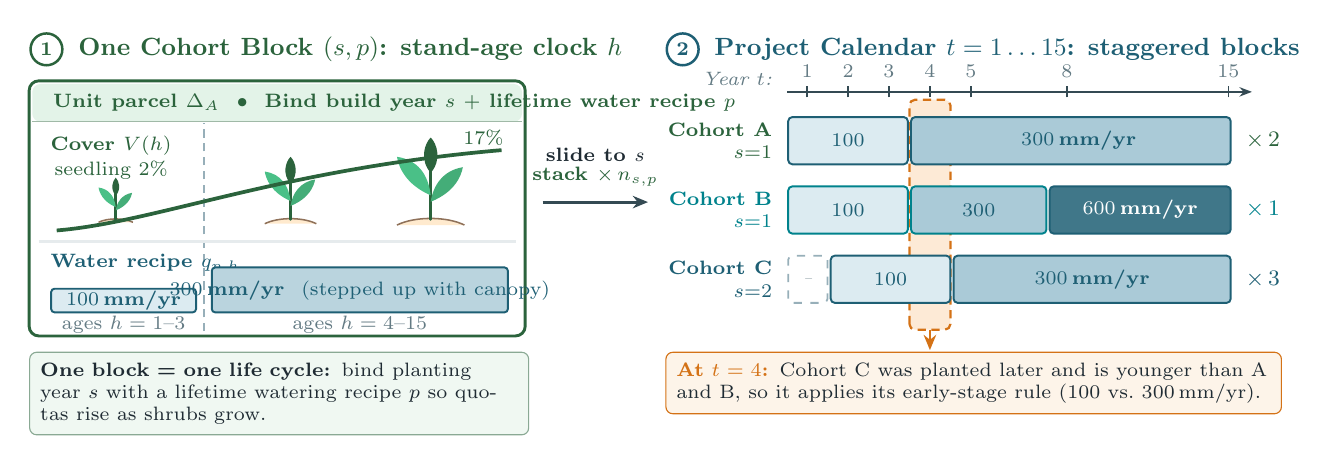
\begin{tikzpicture}[font=\small]

% ======================================================================
% LEFT: (1) One pre-baked Cohort Block (stand-age clock h = 1..15)
% ======================================================================
\node[badge=pVeg] (b1) at (0.22, 3.92) {1};
\node[font=\small\bfseries, text=pVeg, anchor=west] at (0.50, 3.92)
  {One Cohort Block $(s,p)$: stand-age clock $h$};

% Outer card frame
\fill[white, rounded corners=3.5pt] (0, 0.28) rectangle (6.30, 3.52);
\draw[pVeg, line width=1.05pt, rounded corners=3.5pt] (0, 0.28) rectangle (6.30, 3.52);

% Card header bar
\fill[pVegLight, rounded corners=3pt] (0.04, 3.00) rectangle (6.26, 3.48);
\draw[pVeg!45, line width=0.5pt] (0.04, 3.00) -- (6.26, 3.00);
\node[font=\scriptsize\bfseries, text=pVeg, anchor=west] at (0.18, 3.24)
  {Unit parcel $\Delta_A$ \ $\bullet$ \ Bind build year $s$ $+$ lifetime water recipe $p$};

% Age split dashed line at h=3
\draw[pGrey, densely dashed, line width=0.7pt] (2.22, 0.34) -- (2.22, 2.98);

% Top half of card: Shrub growth + Cover V(h) curve
\node[font=\scriptsize\bfseries, text=pVeg, anchor=north west] at (0.15, 2.94) {Cover $V(h)$};
\shrub{1.10}{1.76}{0.52}
\shrub{3.32}{1.76}{0.78}
\shrub{5.10}{1.76}{1.02}
% Smooth rising cover curve
\draw[pVeg, line width=1.35pt] (0.35, 1.62) .. controls (1.6, 1.72) and (3.2, 2.40) .. (6.00, 2.64);
\node[font=\scriptsize, text=pVeg, anchor=west] at (0.20, 2.38) {\scriptsize seedling $2\%$};
\node[font=\scriptsize\bfseries, text=pVeg, anchor=east] at (6.15, 2.80) {$17\%$};

% Divider between vegetation and water recipe inside card
\draw[pGrid, line width=0.8pt] (0.12, 1.48) -- (6.18, 1.48);

% Bottom half of card: Stepped lifetime watering recipe q_{p,h}
\node[font=\scriptsize\bfseries, text=pWater, anchor=north west] at (0.15, 1.45) {Water recipe $q_{p,h}$};
% Age 1-3 low bar (100 mm/yr)
\fill[pWaterLight, draw=pWater, line width=0.7pt, rounded corners=1.2pt] (0.28, 0.58) rectangle (2.12, 0.88);
\node[font=\scriptsize\bfseries, text=pWater] at (1.20, 0.73) {$100$\,mm/yr};
% Age 4-15 higher bar (300 mm/yr)
\fill[pWaterMid!45, draw=pWater, line width=0.7pt, rounded corners=1.2pt] (2.32, 0.58) rectangle (6.08, 1.15);
\node[font=\scriptsize\bfseries, text=pWater] at (4.20, 0.86) {$300$\,mm/yr \ {\normalfont\scriptsize(stepped up with canopy)}};

% Stand-age labels at bottom of card
\node[font=\scriptsize, text=pGreyDark] at (1.20, 0.42) {ages $h=1\text{--}3$};
\node[font=\scriptsize, text=pGreyDark] at (4.20, 0.42) {ages $h=4\text{--}15$};

% Bottom caption under (1)
\node[draw=pVeg!55, fill=pVegLight!55, rounded corners=2.5pt, text width=6.07cm,
      inner sep=3.8pt, font=\scriptsize, text=pInk, anchor=north west] at (0, 0.08)
  {\textbf{One block = one life cycle:} bind planting year $s$ with a lifetime watering recipe $p$ so quotas rise as shrubs grow.};

% ======================================================================
% MIDDLE HANDOFF ARROW
% ======================================================================
\draw[flow=pAxis, line width=1.15pt] (6.52, 1.98) -- (7.86, 1.98);
\node[font=\scriptsize\bfseries, text=pInk, align=center, anchor=south] at (7.19, 2.06)
  {slide to $s$\\[-1pt]{\color{pVeg}stack $\times\,n_{s,p}$}};

% ======================================================================
% RIGHT: (2) Staggered Cohort Blocks on Project Calendar t = 1..15
% ======================================================================
\begin{scope}[xshift=8.08cm]
\node[badge=pWater] (b2) at (0.22, 3.92) {2};
\node[font=\small\bfseries, text=pWater, anchor=west] at (0.50, 3.92)
  {Project Calendar $t=1\dots15$: staggered blocks};

% Calendar header axis
\draw[-{Stealth[length=4.5pt]}, pAxis, line width=0.7pt] (1.55, 3.38) -- (7.45, 3.38);
\foreach \x/\lab in {1.80/1, 2.32/2, 2.84/3, 3.36/4, 3.88/5, 5.10/8, 7.15/15} {
  \draw[pAxis, line width=0.55pt] (\x, 3.31) -- (\x, 3.45);
  \node[font=\scriptsize, text=pGreyDark, anchor=south] at (\x, 3.44) {\lab};
}
\node[font=\scriptsize\itshape, text=pGreyDark, anchor=east] at (1.48, 3.55) {Year $t$:};

% Vertical Year t=4 highlight band BEHIND the tracks
\begin{scope}[on background layer]
  \fill[pAccent!20, rounded corners=2pt] (3.10, 0.36) rectangle (3.62, 3.28);
  \draw[pPV, densely dashed, line width=0.8pt, rounded corners=2pt] (3.10, 0.36) rectangle (3.62, 3.28);
\end{scope}

% Track A: s=1, 100->300, x2 blocks (100 ha)
\node[anchor=east, align=right, font=\scriptsize, text=pVeg] at (1.48, 2.76)
  {\textbf{Cohort A}\\$s{=}1$};
\fill[pWaterLight, draw=pWater, line width=0.7pt, rounded corners=1.5pt] (1.56, 2.46) rectangle (3.08, 3.06);
\node[font=\scriptsize\bfseries, text=pWater] at (2.32, 2.76) {$100$};
\fill[pWaterMid!55, draw=pWater, line width=0.7pt, rounded corners=1.5pt] (3.12, 2.46) rectangle (7.18, 3.06);
\node[font=\scriptsize\bfseries, text=pWater] at (5.25, 2.76) {$300$\,mm/yr};
\node[font=\footnotesize\bfseries, text=pVeg, anchor=west] at (7.25, 2.76) {$\times\,2$};

% Track B: s=1, 100->300->600, x1 block (50 ha)
\node[anchor=east, align=right, font=\scriptsize, text=pTeal] at (1.48, 1.88)
  {\textbf{Cohort B}\\$s{=}1$};
\fill[pWaterLight, draw=pTeal, line width=0.7pt, rounded corners=1.5pt] (1.56, 1.58) rectangle (3.08, 2.18);
\node[font=\scriptsize\bfseries, text=pWater] at (2.32, 1.88) {$100$};
\fill[pWaterMid!55, draw=pTeal, line width=0.7pt, rounded corners=1.5pt] (3.12, 1.58) rectangle (4.84, 2.18);
\node[font=\scriptsize\bfseries, text=pWater] at (3.98, 1.88) {$300$};
\fill[pWater!85, draw=pWater, line width=0.7pt, rounded corners=1.5pt] (4.88, 1.58) rectangle (7.18, 2.18);
\node[font=\scriptsize\bfseries, text=white] at (6.03, 1.88) {$600$\,mm/yr};
\node[font=\footnotesize\bfseries, text=pTeal, anchor=west] at (7.25, 1.88) {$\times\,1$};

% Track C: s=2 (shifted by 1 year!), 100->300, x3 blocks (150 ha)
\node[anchor=east, align=right, font=\scriptsize, text=pWater] at (1.48, 1.00)
  {\textbf{Cohort C}\\$s{=}2$};
\draw[pGrey, dashed, line width=0.65pt, rounded corners=1.5pt] (1.56, 0.70) rectangle (2.06, 1.30);
\node[font=\tiny\itshape, text=pGreyDark] at (1.81, 1.00) {--};
\fill[pWaterLight, draw=pWater, line width=0.7pt, rounded corners=1.5pt] (2.10, 0.70) rectangle (3.62, 1.30);
\node[font=\scriptsize\bfseries, text=pWater] at (2.86, 1.00) {$100$};
\fill[pWaterMid!55, draw=pWater, line width=0.7pt, rounded corners=1.5pt] (3.66, 0.70) rectangle (7.18, 1.30);
\node[font=\scriptsize\bfseries, text=pWater] at (5.42, 1.00) {$300$\,mm/yr};
\node[font=\footnotesize\bfseries, text=pWater, anchor=west] at (7.25, 1.00) {$\times\,3$};

% Arrow from the Year t=4 slice down to the linear sum explanation
\draw[flow=pPV] (3.36, 0.36) -- (3.36, 0.10);

% Bottom takeaway box under (2)
\node[draw=pPV, fill=pPVLight!80, rounded corners=2.5pt, text width=7.55cm,
      inner sep=3.8pt, font=\scriptsize, text=pInk, anchor=north west] at (0, 0.08)
  {{\color{pPV}\textbf{At $t=4$:}} Cohort~C was planted later and is younger than A and B, so it applies its early-stage rule ($100$ vs.\ $300$\,mm/yr).};
\end{scope}

\end{tikzpicture}
\end{document}
